\capitulo{4}{Techniques and tools}

The objective of this part of the project is to present the methodological techniques and development tools used in the project's development.

\section{Tools}
\begin{itemize}
\item Python: Python is a high-level programming language widely used in the field of machine learning and artificial intelligence. It has a high number of libraries and frameworks that facilitate data processing and implementation of artificial intelligence algorithms.
In this project it has been used to develop all the back-end part of the application.

\item librosa: librosa is a Python library used for audio analysis and processing. It provides a wide range of methods to extract audio features in a simple way. Some examples are spectrograms, mel frequency cepstral coefficients (MFCC) or chromagrams.
In this project it has been used to process and extract various audio features to feed the artificial intelligence algorithms and create the model.

\item TensorFlow: TensorFlow is an open source library used in the field of machine learning. It provides a simple interface for the implementation of neural networks and other machine learning algorithms.
TensorFlow has been the chosen option to train the neural network algorithms of the project.

\item scikit-learn: scikit-learn is a Python machine learning library that provides a wide range of algorithms and tools for data analysis and model building. Includes functions for splitting datasets into \textit{train} and \textit{test}.

\item NumPy: NumPy is a Python library used to perform numerical calculations on matrices and multidimensional arrays. It provides a wide range of mathematical functions and tools for efficient handling of numerical data.

\item Pandas: open source Python library that provides data analysis tools. It is very used in data science fields.
\end{itemize}

\section{Justification}

\subsection{Python}
The following includes some of the justifications that have led to the development of the project in Python language compared to other languages.

\textbf{Extensive variety of libraries and frameworks}: Python has a broad range of libraries and frameworks specialized in machine learning, such as TensorFlow, scikit-learn, PyTorch, Keras and many others. 
These libraries provide tools and implementation of the main artificial intelligence algorithms, which facilitates the task of developing a machine learning project.

\textbf{Integration with other technologies}: Python easily integrates with other existing technologies in machine learning development area. For example, it can be combined with relational databases (MySQL), visualization tools (matplotlib, Seaborn), data analysis (Pandas) or in this case, music processing tools (librosa).

\subsection{TensorFlow vs scikit-learn}
The choice to use TensorFlow instead of scikit-learn is based on several considerations.

\textbf{First}, TensorFlow is suitable for projects involving deep learning and neural networks. It provides a higher number of tools for creating, training, and deploying deep learning models than scikit-learn. 

\textbf{TensorFlow} allows implementing complex neural network architectures, such as convolutional neural networks (CNNs), which are particularly well suited for this project.

\textbf{Finally}, TensorFlow supporst graphics cards (GPUs) to perform the training process. This provides a very significant performance advantage, as the large number of cores in a GPU can be used to perform parallel and distributed computations. The result is a considerably faster training time compared to a GPU.

\section{Techniques}

Several techniques and methodologies have been used to develop and train the machine learning models.

(A much more detailed description of the methodological development of the project can be found in the document \textit{Annexes}).

\section{Processing and extracting audio features}

librosa has been used for the audio processing and features extraction.

\begin{itemize}
\item MFCC (mel frequency cepstral coefficients): These coefficients capture the spectral features of audio and are commonly used in speech recognition and audio classification tasks. They are the main features that have been used to train the model and make predictions.
\end{itemize}

\section{Dataset splitting}

scikit-learn library has been used to split the dataset into training, test and validation data.
Scikit-learn provides a function called \textit{train\textunderscore test\textunderscore split} that splits the dataset into parts intended for training and model evaluation. 
This data set splitting technique is critical to evaluate the model's generalizability and to avoid overfitting.

\begin{figure}
  \centering
  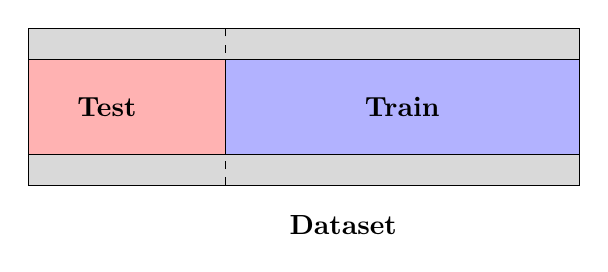
\begin{tikzpicture}
    % Width of training and test sets
    \def\datasetwidth{6}
    
    % dataset
    \draw[fill=gray!30] (-1,0) rectangle (\datasetwidth,2);
    
    % test
    \draw[fill=red!30] (-1,0.4) rectangle (1.5,1.6);
    \node at (0,1) {\textbf{Test}};
    
    % train
    \draw[fill=blue!30] (1.5,0.4) rectangle (\datasetwidth,1.6);
    \node at (3.75,1) {\textbf{Train}};
    
    \draw[dashed] (1.5,0) -- (1.5,2);
    
    \draw[dashed] (-1,0.4) -- (\datasetwidth,0.4);
    \draw[dashed] (-1,1.6) -- (\datasetwidth,1.6);
    
    % Etiqueta del conjunto completo
    \node at (\datasetwidth/2,-0.5) {\textbf{Dataset}};
  \end{tikzpicture}
  \caption{Dataset splitting}
\end{figure}

\section{Neural networks with TensorFlow}

Neural networks implemented with TensorFlow library have been used to train the data.

In this project, various neural network architectures have been used, such as convolutional neural networks (CNN) and multilayer neural networks. These architectures are suitable for audio processing tasks and have proven to be effective in audio classification and pattern recognition.

Neural networks are trained by updating the weights and biases of the network iteratively to minimize \textit{loss}. Once trained, neural networks make predictions on new audio data, classifying them into categories or musical styles.

\begin{figure}
  \centering
  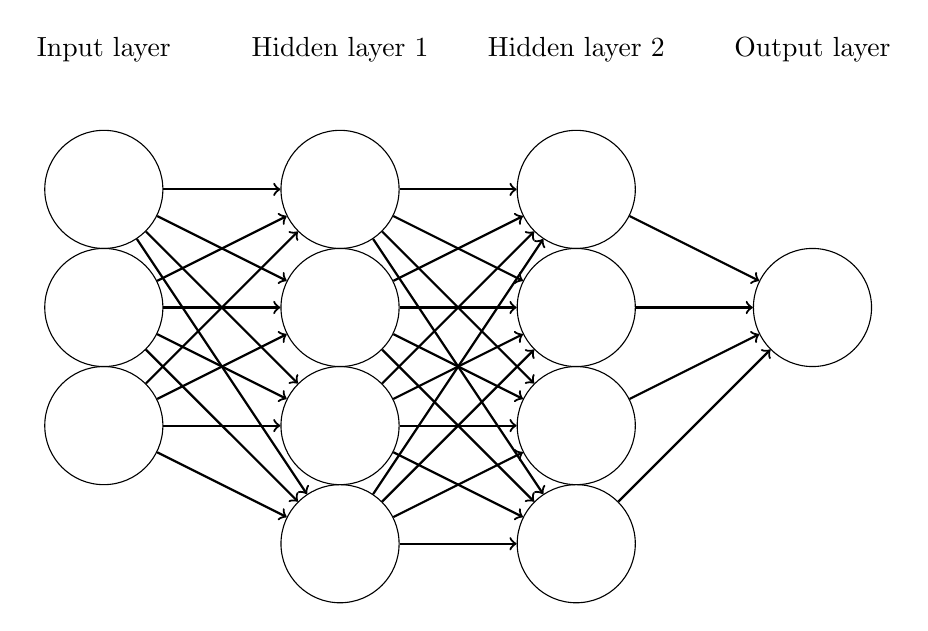
\begin{tikzpicture}[
    neuron/.style={circle, draw, minimum size=1.5cm},
    connection/.style={->, thick}
  ]
    % Input layer
    \foreach \i in {1,2,3}
      \node[neuron] (input\i) at (0,-\i*1.5) {};

    % Hidden layer 1
    \foreach \i in {1,2,3,4}
      \node[neuron] (hidden1\i) at (3,-\i*1.5) {};

    % Hidden layer 2
    \foreach \i in {1,2,3,4}
      \node[neuron] (hidden2\i) at (6,-\i*1.5) {};

    % Output layer
    \node[neuron] (output) at (9, -3) {};

    % Connections
    \foreach \i in {1,2,3}
      \foreach \j in {1,2,3,4}
        \draw[connection] (input\i) -- (hidden1\j);

    \foreach \i in {1,2,3,4}
      \foreach \j in {1,2,3,4}
        \draw[connection] (hidden1\i) -- (hidden2\j);

    \foreach \i in {1,2,3,4}
      \draw[connection] (hidden2\i) -- (output);

    \node[above] at (0,0) {Input layer};
    \node[above] at (3,0) {Hidden layer 1};
    \node[above] at (6,0) {Hidden layer 2};
    \node[above] at (9,0) {Output layer};

  \end{tikzpicture}
  \caption{Multi-layer neural network example}
\end{figure}

\section{Development with Python and Flask}

Web application development part was implemented using Python and the Flask framework. Flask is a web framework that allows building web applications in Python.

The back-end of the application has been developed in Flask, which is responsible for receiving user requests, processing audio data and returning classification and analysis results. 
All this through the implementation of RESTful API, which provides continuous communication between the user and the server.

